\documentclass{beamer}
\usepackage{amsfonts, amsmath, graphicx, verbatim, graphicx, hyperref,
  color}
\definecolor{UNBlue}{RGB}{91, 146, 229}
\setbeamercolor{structure}{fg=UNBlue}
\newcommand\Fontvi{\fontsize{6.5}{7.2}\selectfont}
\usetheme{Warsaw}

\title{Statistical Standardization of the Supply and Utilization Accounts}
\author{\it Michael C. J. Kao}
\institute{Economic and Social Statistics Division (ESSD)\\ \vspace{0.1in} Food and Agriculture Organization \\ of the United Nations}

\date{}

\AtBeginSection[]
{
  \begin{frame}<beamer>
    \frametitle{Outline for section \thesection}
    \tableofcontents[currentsection]
  \end{frame}
}

\begin{document}

\frame{
  \titlepage
  \centering
  
\includegraphics[scale = 0.2]{fao_logo.png}
}

\frame{
  \frametitle{Outline}
  \tableofcontents
}


\section{Introduction}
%% \frame{
%%   \frametitle{Introduction}

%%   The Food Balance Sheets (FBS) detail this statistic with information
%%   on commodity groups. Creating the FBS from the SUAs amounts to an
%%   aggregation process where input use of primary products is cancelled
%%   out against the production of derived products. Within the
%%   Organisation this process is referred to as "standardisation".

%% }

\frame{
  \frametitle{What is standardization}

  Standardization in this context is the process of converting
  processed commodity to a standard expression for comparison both in
  terms of \textbf{calorie} and \textbf{quantity}.

}

\frame{
  \frametitle{Commodity Tree Mapping}
  
  To perform standardization, one must specify the relationship
  between the elements, one such instance is the commodity tree. The
  current specification is technically known as a \textbf{rooted
    tree}.

  \vfill

  A rooted tree is a tree which has a designated vertex known as the
  \textbf{root}. In the context of standardization, it is the primary
  commodity group or the unit group we would like to standardize
  to. 

}

\frame{

  \begin{figure}
    \centering
    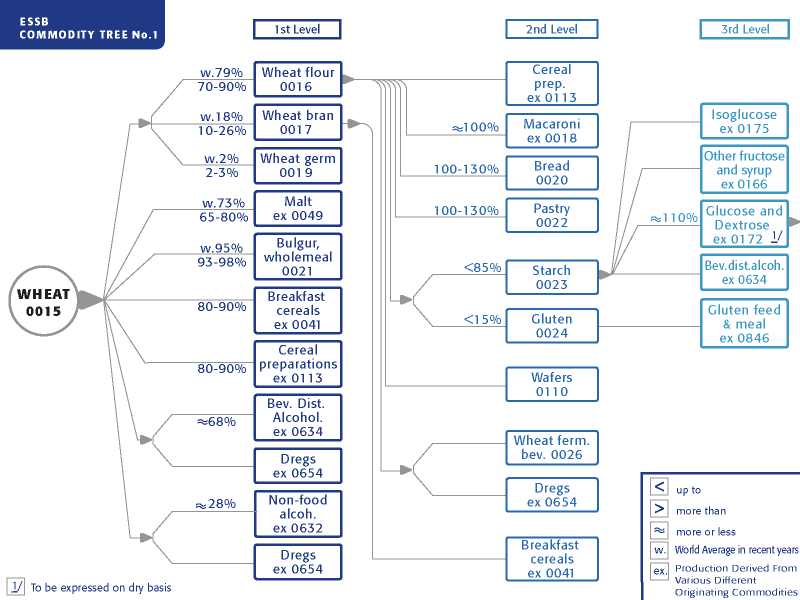
\includegraphics[scale = 0.3]{wheat_commodity_tree.png}
  \end{figure}

}



\section{Theory}
\frame{
  \frametitle{Background}

  The tree is intuitive but restrictive, in this seminar we
  would like to propose the more general flexible framework of graph
  for standardization.

}

\frame{
  \frametitle{Terminology}
  \begin{itemize}
    \setlength{\itemindent}{1in}
    \item[Vertex: ] A node representing the commodity
    \item[Edge: ] A line connecting the vertex.
    \item[Root: ] A specific designated node.
    \item[Parent: ] The node directly above the other node.
    \item[Leaf: ] A node which has has no child.
  \end{itemize}
  
}

\frame{

  In a rooted tree, a vertex can have and at most one \textit{parent},
  we would like to relax this and allow multiple inputs for each
  derivative.

  \vfill

  Furthermore, we don't want to fix the selection of the root. We want
  to be flexible and be able to standardize to any equivalence. To
  achieve this, we need the vertex to be able to reach every single
  other vertex.

}

\frame{
  \frametitle{This is more than a graph, its a mathematical model}
  \begin{figure}
    \centering
    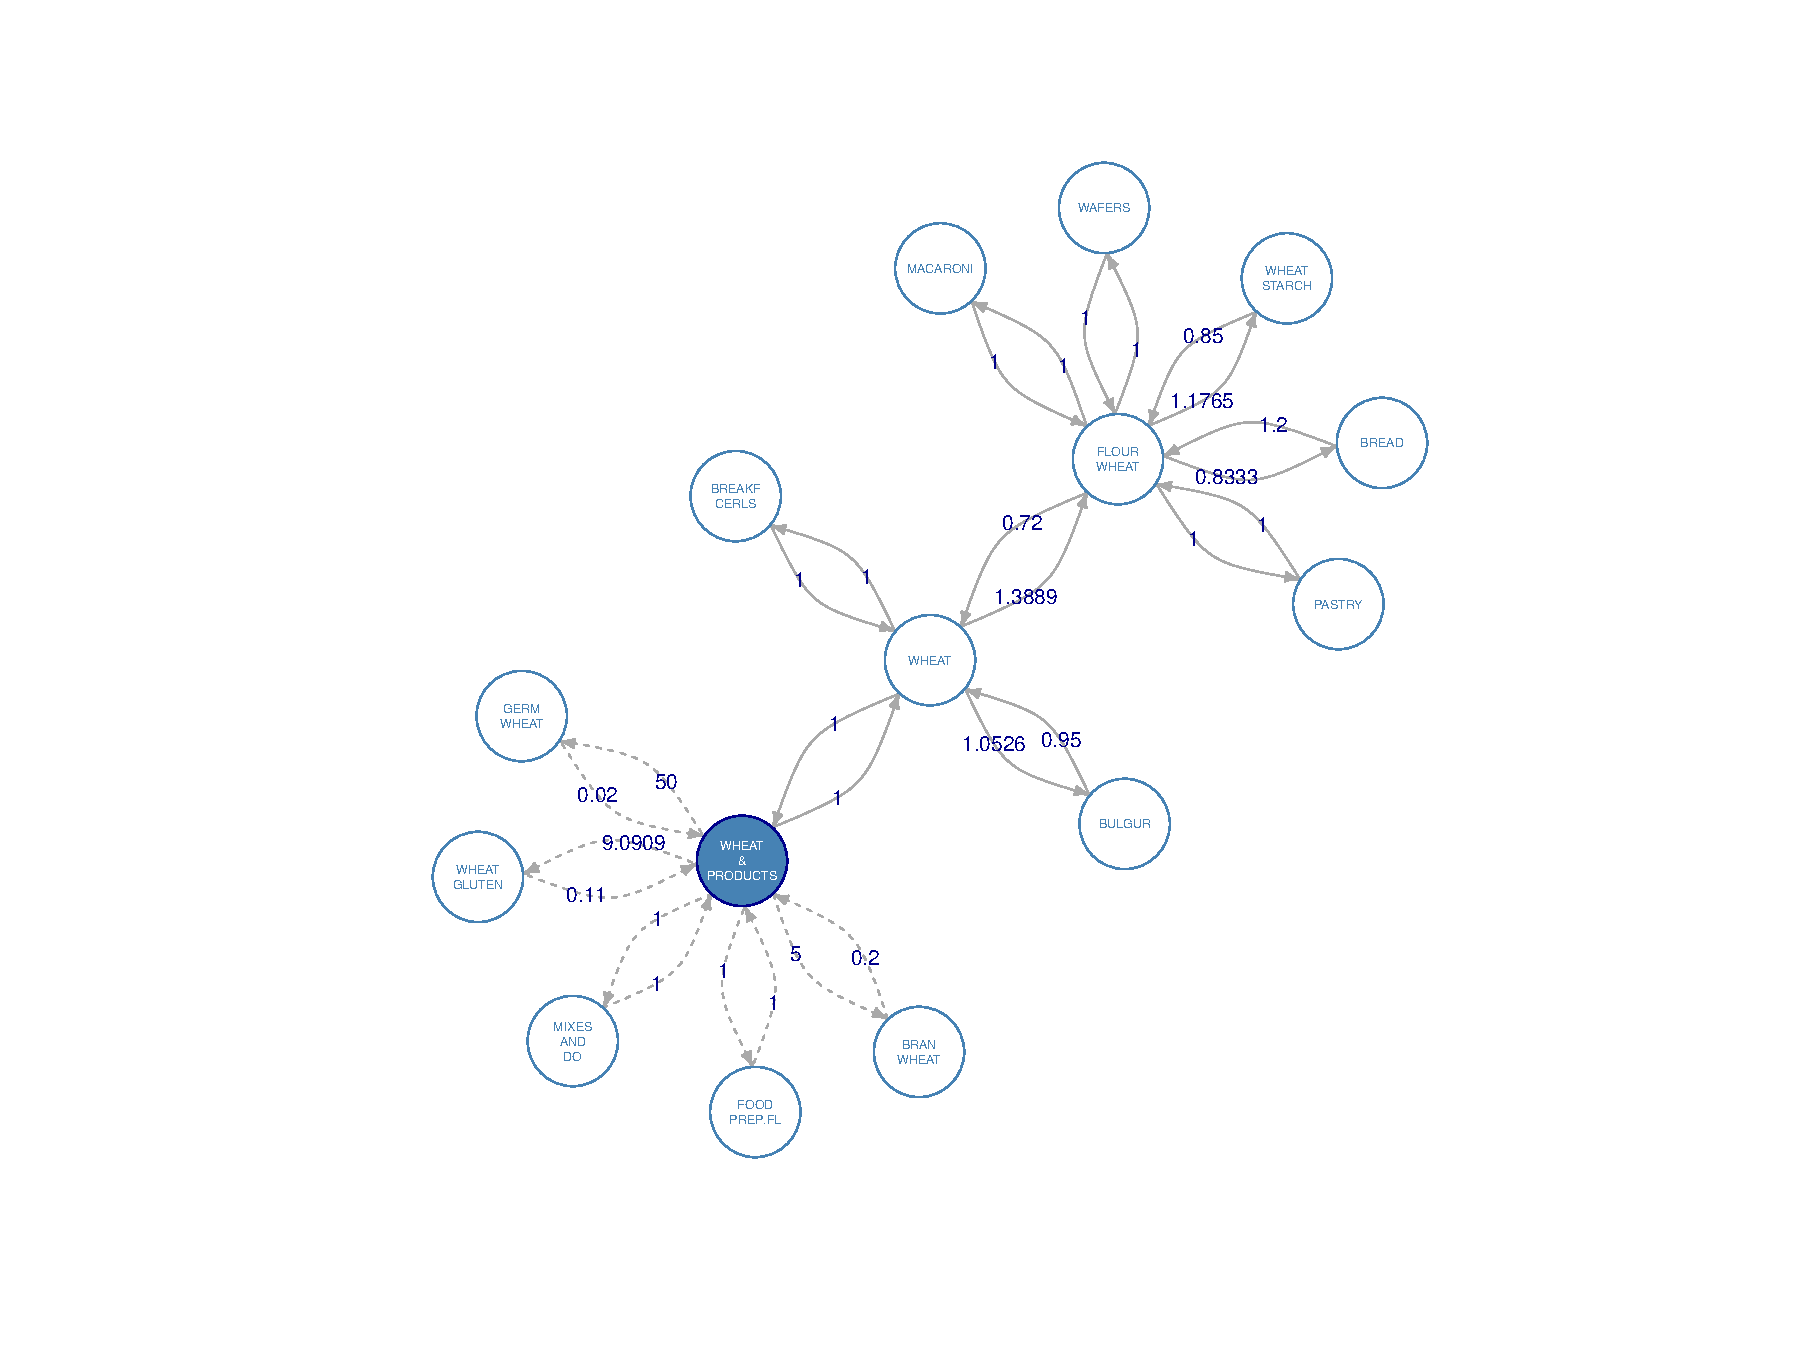
\includegraphics[scale = 0.33]{wheat_network.pdf}
  \end{figure}

}
\frame{
  \frametitle{Benefits of a network specification}
  
  \begin{itemize}
    \setlength{\itemindent}{1in}
    \item[Traceability: ] We can see how it is standardized.
    \item[Flexibility:] It can take every single possible form.
    \item[Easibility: ] The specification can be handled easily.
  \end{itemize}
}


\section{Traditional Accounting Standardization}

\frame{

  Tradtional accounting standardization system assume that everything
  is measured without error, and the standardization process is merely
  a matrix arithematic exercise.

  \vfill

  This is both unrealistic in practice and problematic as we
  over-state our confidence about the estimates.

}

\section{Statistical Standardization of the SUA}

\frame{

  To account for this over-simplified scenario, we propose to use a
  statistical framework for standardization.

  \vfill

  Quantities can be specified as distribution to reflect uncertainty
  or lack of state of knowledge. 


}

\frame{
  %% \frametitle{Analytical Standardization}  

  Take the commodity tree for example, the extract rate of wheat flour
  from wheat is between $70 \sim 90\%$ with a global average of
  79\%. This can be represented as a normal distribution with mean of
  0.79 and a standard deviation of 0.035.

  \vfill

  The result of the standardization will then be expressed in the
  primary equivalent with mean ($\mu$) equivalent to the accounting
  system but a distribution reflecting the lack of information.



}

\frame{
  \frametitle{Analytical Standardization}

  The next page shows a distributional standardization based on the
  normal distribution. We have add uncertainty to the quantity of
  \textbf{Wheat Flour} and \textbf{Bread}, the standardization shows
  that the final group \textbf{wheat and Products} now has a normal
  distritbution as well.

  \begin{align}
    \text{Let:} \hspace{80pt}& \nonumber\\
    \text{Bread} &\sim \mathcal{N}(\mu_{\text{bread}}, \sigma_{\text{bread}})\nonumber \\
    \text{Wheat flour} &\sim \mathcal{N}(\mu_{\text{wheat flour}}, \sigma_{\text{wheat flour}}) \nonumber\\
    \text{then: } \hspace{70pt}& \nonumber\\
    \text{Wheat and Products} &\sim \mathcal{N}\left(\sum_{i \in \mathcal{C}} \mu_{i}, \sqrt{\sum_{i \in \mathcal{C}} \sigma_{i}^2}\right) \nonumber
  \end{align}


}

\frame{
  \frametitle{Analytical Standardization}

  \begin{figure}
    \centering
    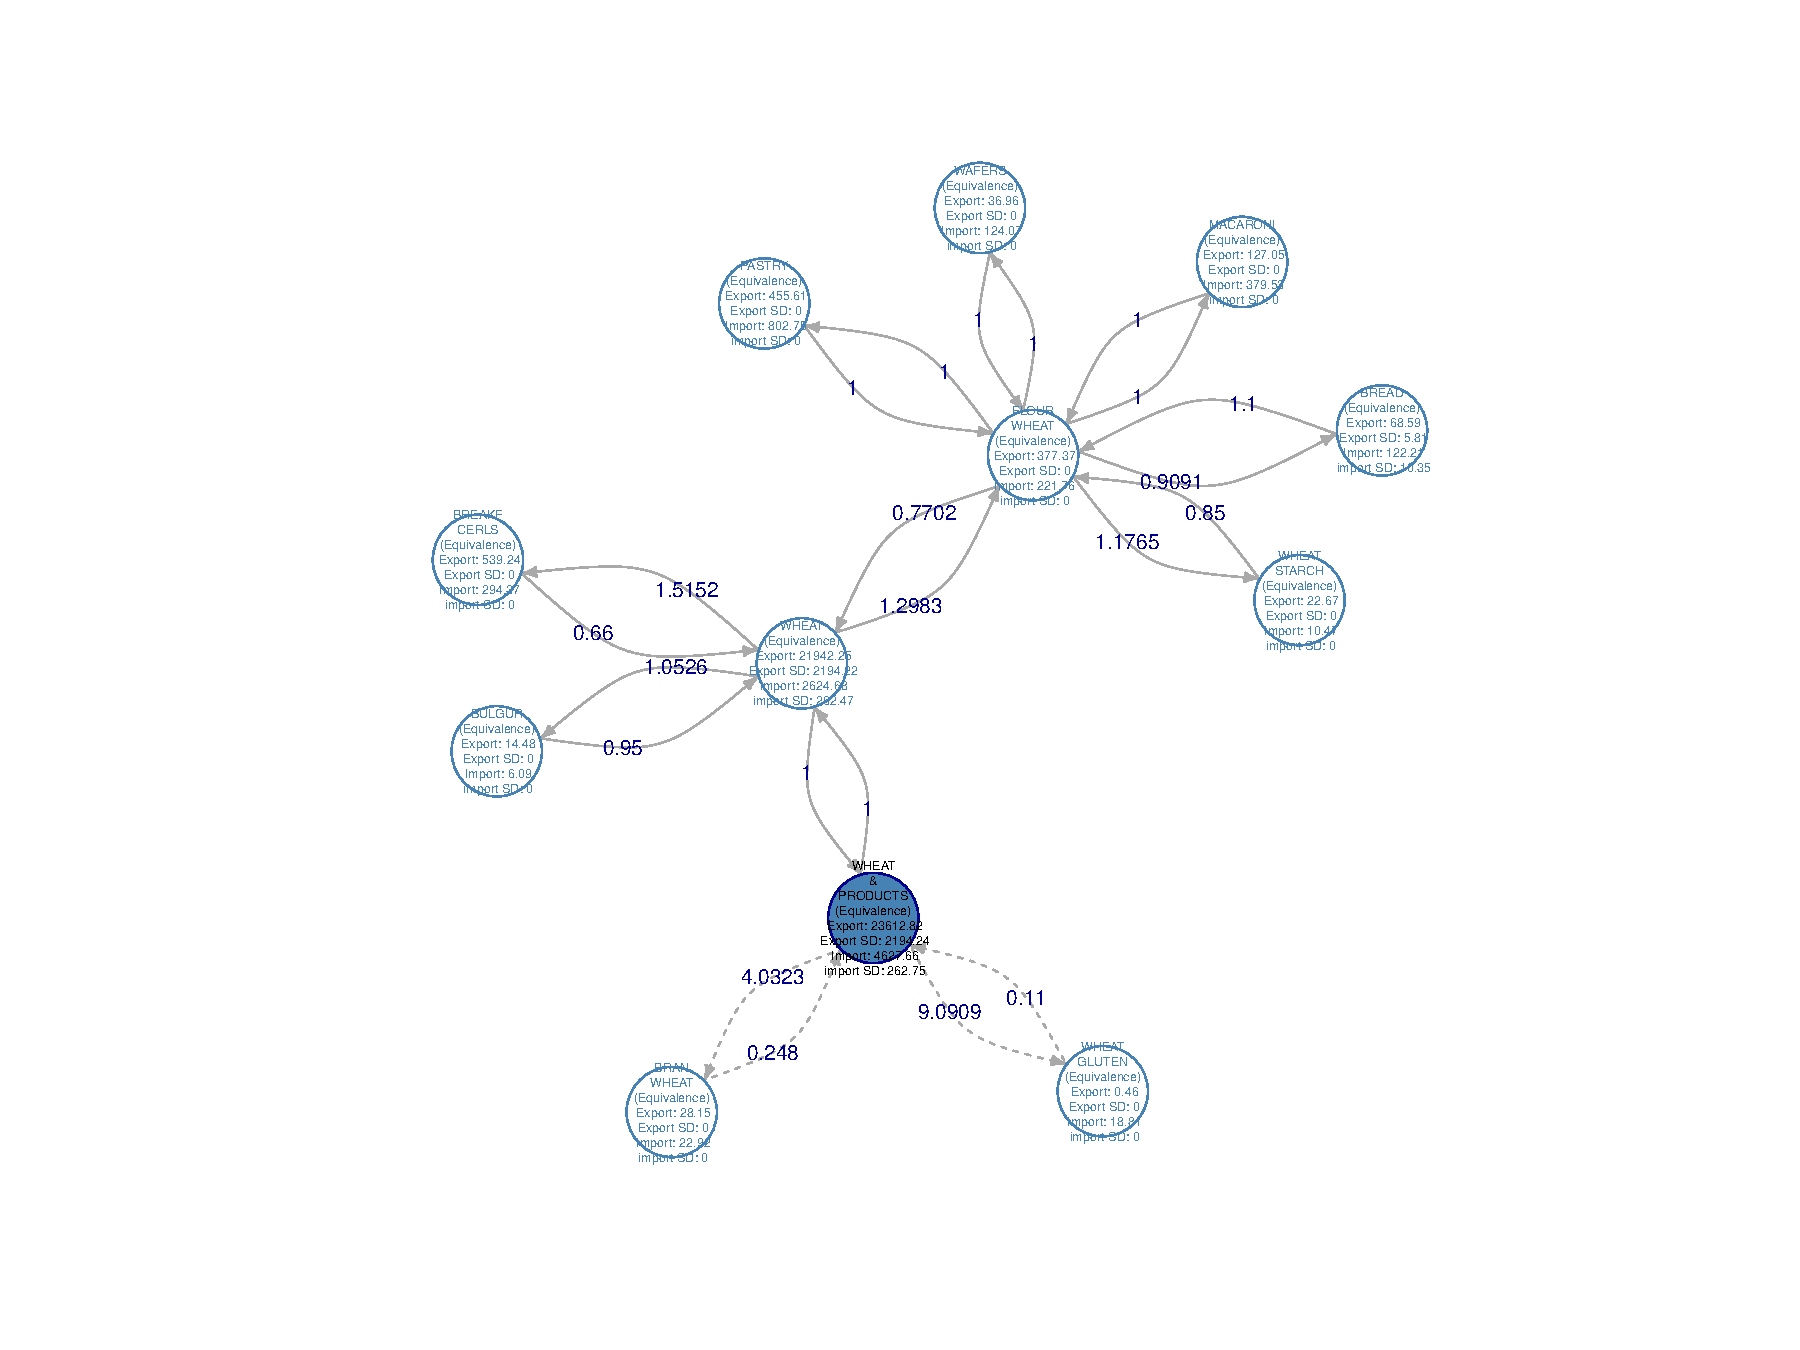
\includegraphics[scale = 0.33]{wheat_usa_2009_distribution_standardized_network.pdf}
  \end{figure}  
}


\frame{
  \frametitle{MCMC Standardization}

  We don't have to restrict ourself to distribution with analytical
  posterior, as a matter of fact we can speficy any distribution and
  obtain the posterior via MCMC.

  \vfill
  
  We can model the dependency between extraction rate and calorie at
  the same time, and many other joint probability.

}

\frame{
  \frametitle{MCMC Standardization}
  
  Let us assume the following complicated situation:
  \begin{align}
    \text{wheat} &\sim \mathcal{U}\left(E_{a, b}, \sum_{i \in \mathcal{T}} I_{b, a}\right)\nonumber \\
    \text{bread} &\sim \mathcal{U}\left(E_{a, b}, \sum_{i \in \mathcal{T}} I_{b, a}\right)\nonumber \\
    \text{Wheat flour \& Bulgur} &\sim \mathcal{N}(\boldsymbol{\mu}, \boldsymbol{\Sigma}) \nonumber\\
    \text{Pastry} &\sim \Gamma(\alpha, \beta) \nonumber
  \end{align}  
 
}

\frame{
  \frametitle{Posterior distribution of wheat equivalent}

  \begin{figure}
    \centering
    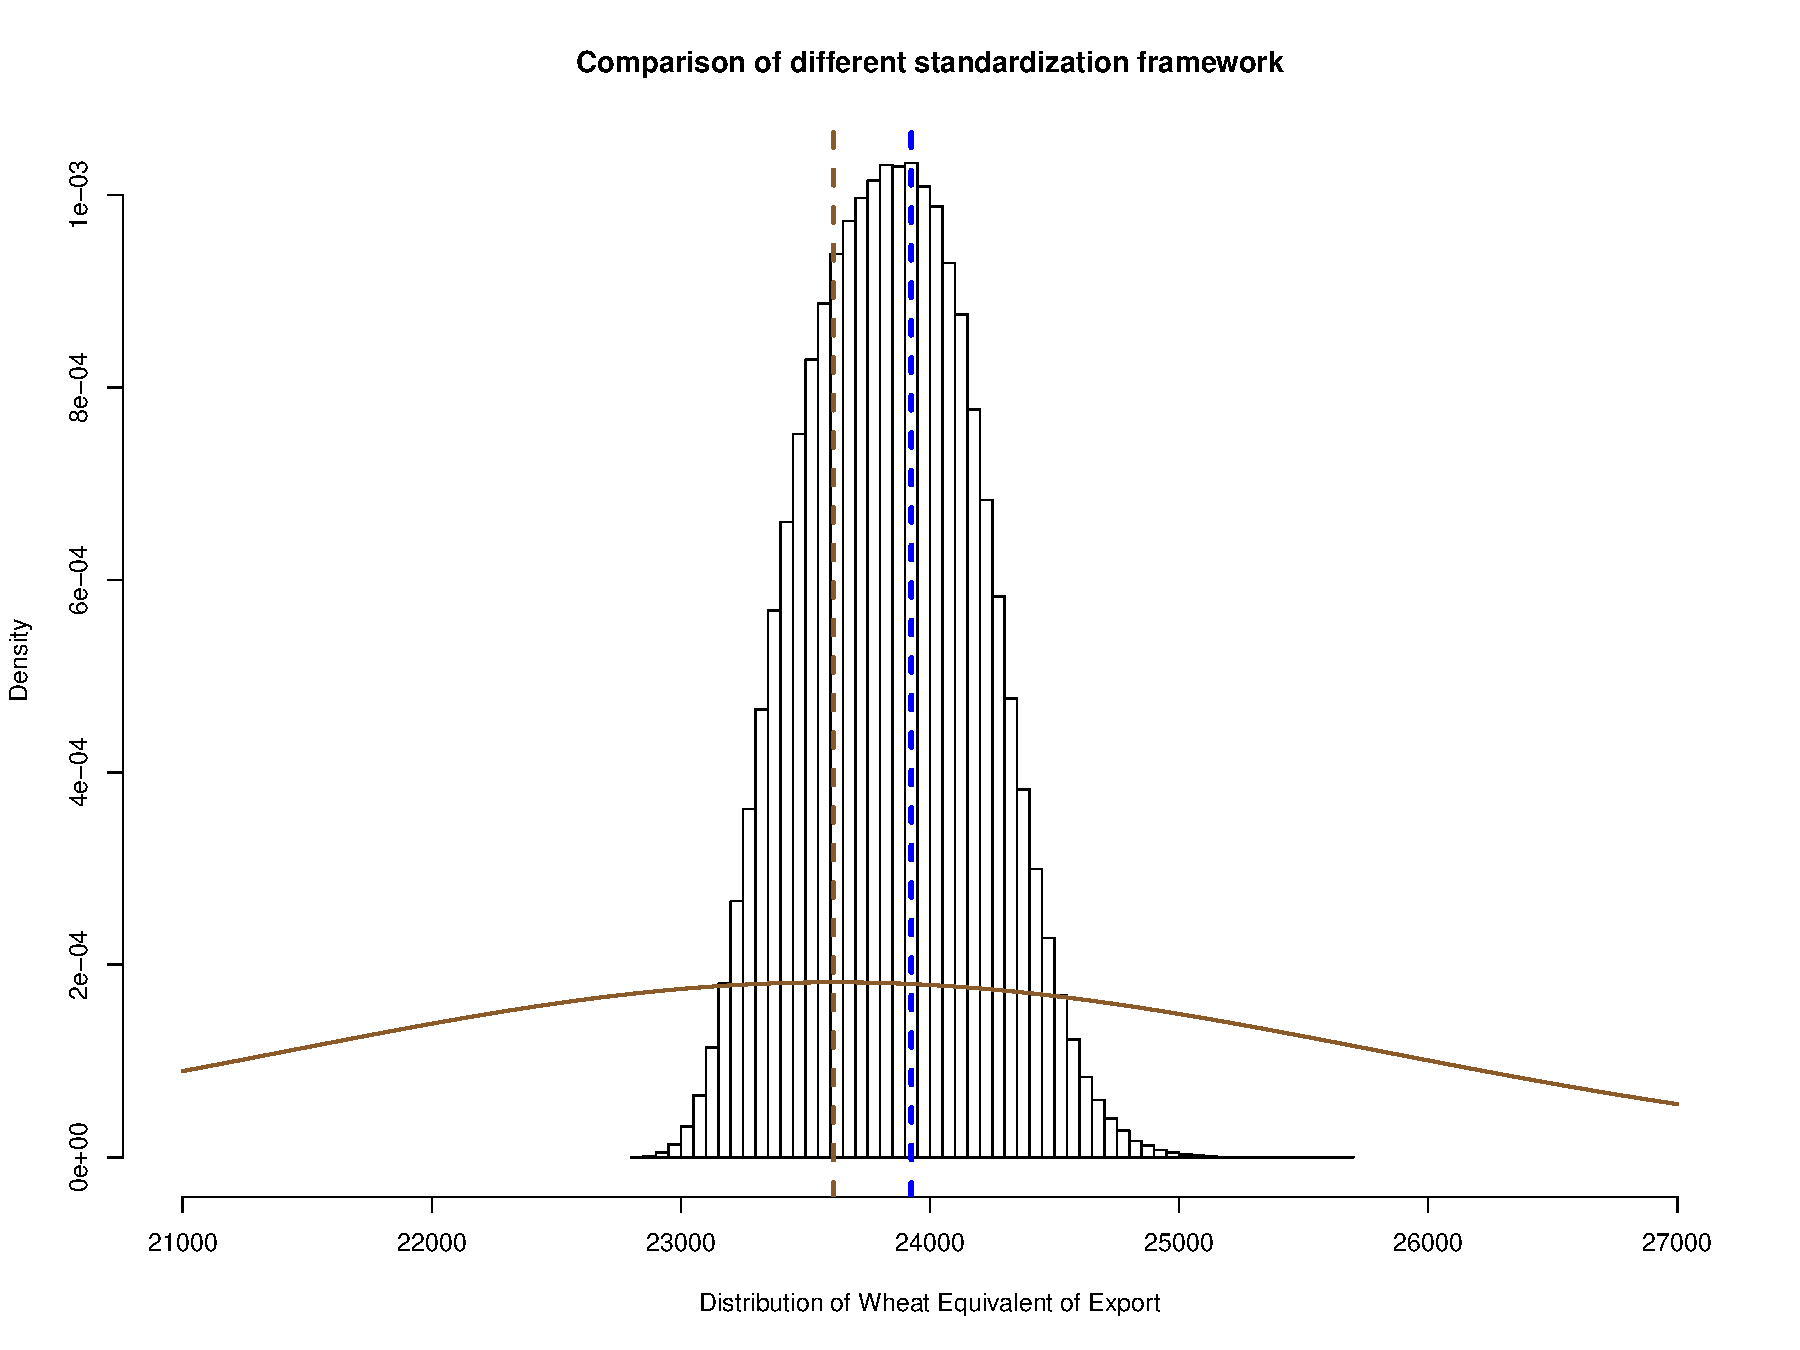
\includegraphics[scale = 0.3]{wheat_mcmc_standardization.pdf}
  \end{figure}    
}

%% \frame{
%%   \frametitle{Bayesian Network Standardization}

%%   Furthermore, we can specify the network as a Bayesian network to
%%   model the dependency in the distributions.

%%   For example, if the extraction rate of wheat flour is 90\% then we
%%   known the wheat flour may contain traces of bran or germ and thus
%%   has a different calorie content.

%% }

\section{Implications}

\frame{
  \frametitle{Calibration of quantity and calorie}

  There may be potentital ways of calibrate the two in a single model.

}


%% \frame{
%%   \frametitle{Reconciliation of Trade}  
%% }

\frame{
  \frametitle{Integration with the new FBS balancing methodology}
  
  The new standardization provides a lower level prior distribution
  for the multiway-contingency sampling in the new FBS balancing
  methodology. 
  
  \vfill

  It give us more insight about the sources of the variability and
  undertainty rather than guess at the aggregated level.

}

\frame{
  \frametitle{Bayesian estimate of the Prevalence of Undernourishment}

  The calorie computed from the standardization and ultimately the
  dietary energy supply (DES) is used for the calculation of the
  Prevalence of Undernourishment (PoU). 

  \vfill

  Bayesian methodology can be developed for PoU to reflect our
  uncertainty about food availability.

}

\section{Further Work}
\frame{
  \frametitle{How to set the prior distribution?}
  
  Given the large number of commodity, it may be difficult to set the
  prior distribution for all the elements accross all country for the
  whole system.

  \vfill

  It may be possible to estimate the prior distribution via the use of
  maximum entropy to formulate a full objective Bayesian framework,
  but also allow the possibility for human intervention.

}



%% \begin{frame}[allowframebreaks]
%%   \frametitle{Reference}
%%   \begin{thebibliography}{10}
%%   \end{thebibliography}
%% \end{frame}
  

\end{document}
